%!TeX program = xelatex
\documentclass[useamsfonts]{pasj01}
\draft
\usepackage{latexsym}%,amssymb}
\usepackage{natbib,amssymb}
\usepackage{amsmath}

\usepackage{url}

\newcommand \redColor{}%\color{red}}
\newcommand \bColor{}%\color{blue}}
\newcommand \oColor{}%\color{orange}}
\renewcommand\labelenumi{(\roman{enumi})}
\renewcommand\theenumi\labelenumi
\renewcommand{\vec}[1]{\boldsymbol{#1}}

\newcommand{\galsim}{\texttt{GalSim}}
\newcommand{\sersic}{{S\'ersic}}
\newcommand{\res}{\mathcal {R}}

\newcommand{\mtrv}[1]{#1}
\newcommand{\rmrv}[1]{#1}
\newcommand{\hmrv}[1]{#1}
\newcommand{\smrv}[1]{#1}


\begin{document}


\title{}
\author{}%
\altaffiltext{}{}
\email{}

\KeyWords{Cosmology, Weak Gravitational Lensing, Image Processing}

\maketitle


\begin{abstract}
\end{abstract}

\section{Introduction}
\label{sec:Intro}

\section{HSC Data and Pipeline}
\label{sec:DataPipe}
\begin{enumerate}
    \item seeing maps
    \item Nexp maps: check the difference between Nexp from FDFC and that from countInput.
    \item residual size maps
    \item residual size vs seeing
    \item seeing distributions: S16A vs S19A
    \item number density map (together with positions of PSFs used for image simulations, we should mention the bad visit in GAMA09H).
    \item weighted number density map
    \item number density vs seeing
%    \item maps of the S16A and the S19A star mask
\end{enumerate}

\subsection{S19A data release}
\subsubsection{Selections}

\subsubsection{FDFC cut}

\subsubsection{5 dither vs 6 dither}

\subsection{HSC pipline 7}
\subsubsection{Warping}

\subsubsection{Bright star mask}

\subsubsection{Background subtraction}

\subsubsection{reGaussianization shear estimator}


\section{Requirement}
\label{sec:Requirement}

\subsection{Covariance}

\subsection{Galaxy-galaxy Lensing}

\subsection{Cosmic Shear}


\section{PSF Model Test}
\label{sec:psftest}
\begin{enumerate}
    \item magnitude distribution of PSF stars and non PSF stars
    \item residual size distribution of PSF stars and non-PSF stars
    \item residual size vs magnitude: PSF stars vs non-PSF stars
    \item residual size vs binned seeing
    \item residual size correlation
    \item residual shape distributions
    \item rho statistics
\end{enumerate}
\subsection{Median vs Mean}

\subsection{PSF stars vs Non-PSF stars}
% Eli's star catalog

\subsection{Simulation}
\label{sec:Sim}

\subsubsection{Noise and PSF}


\begin{figure*}[ht!]
\centering{
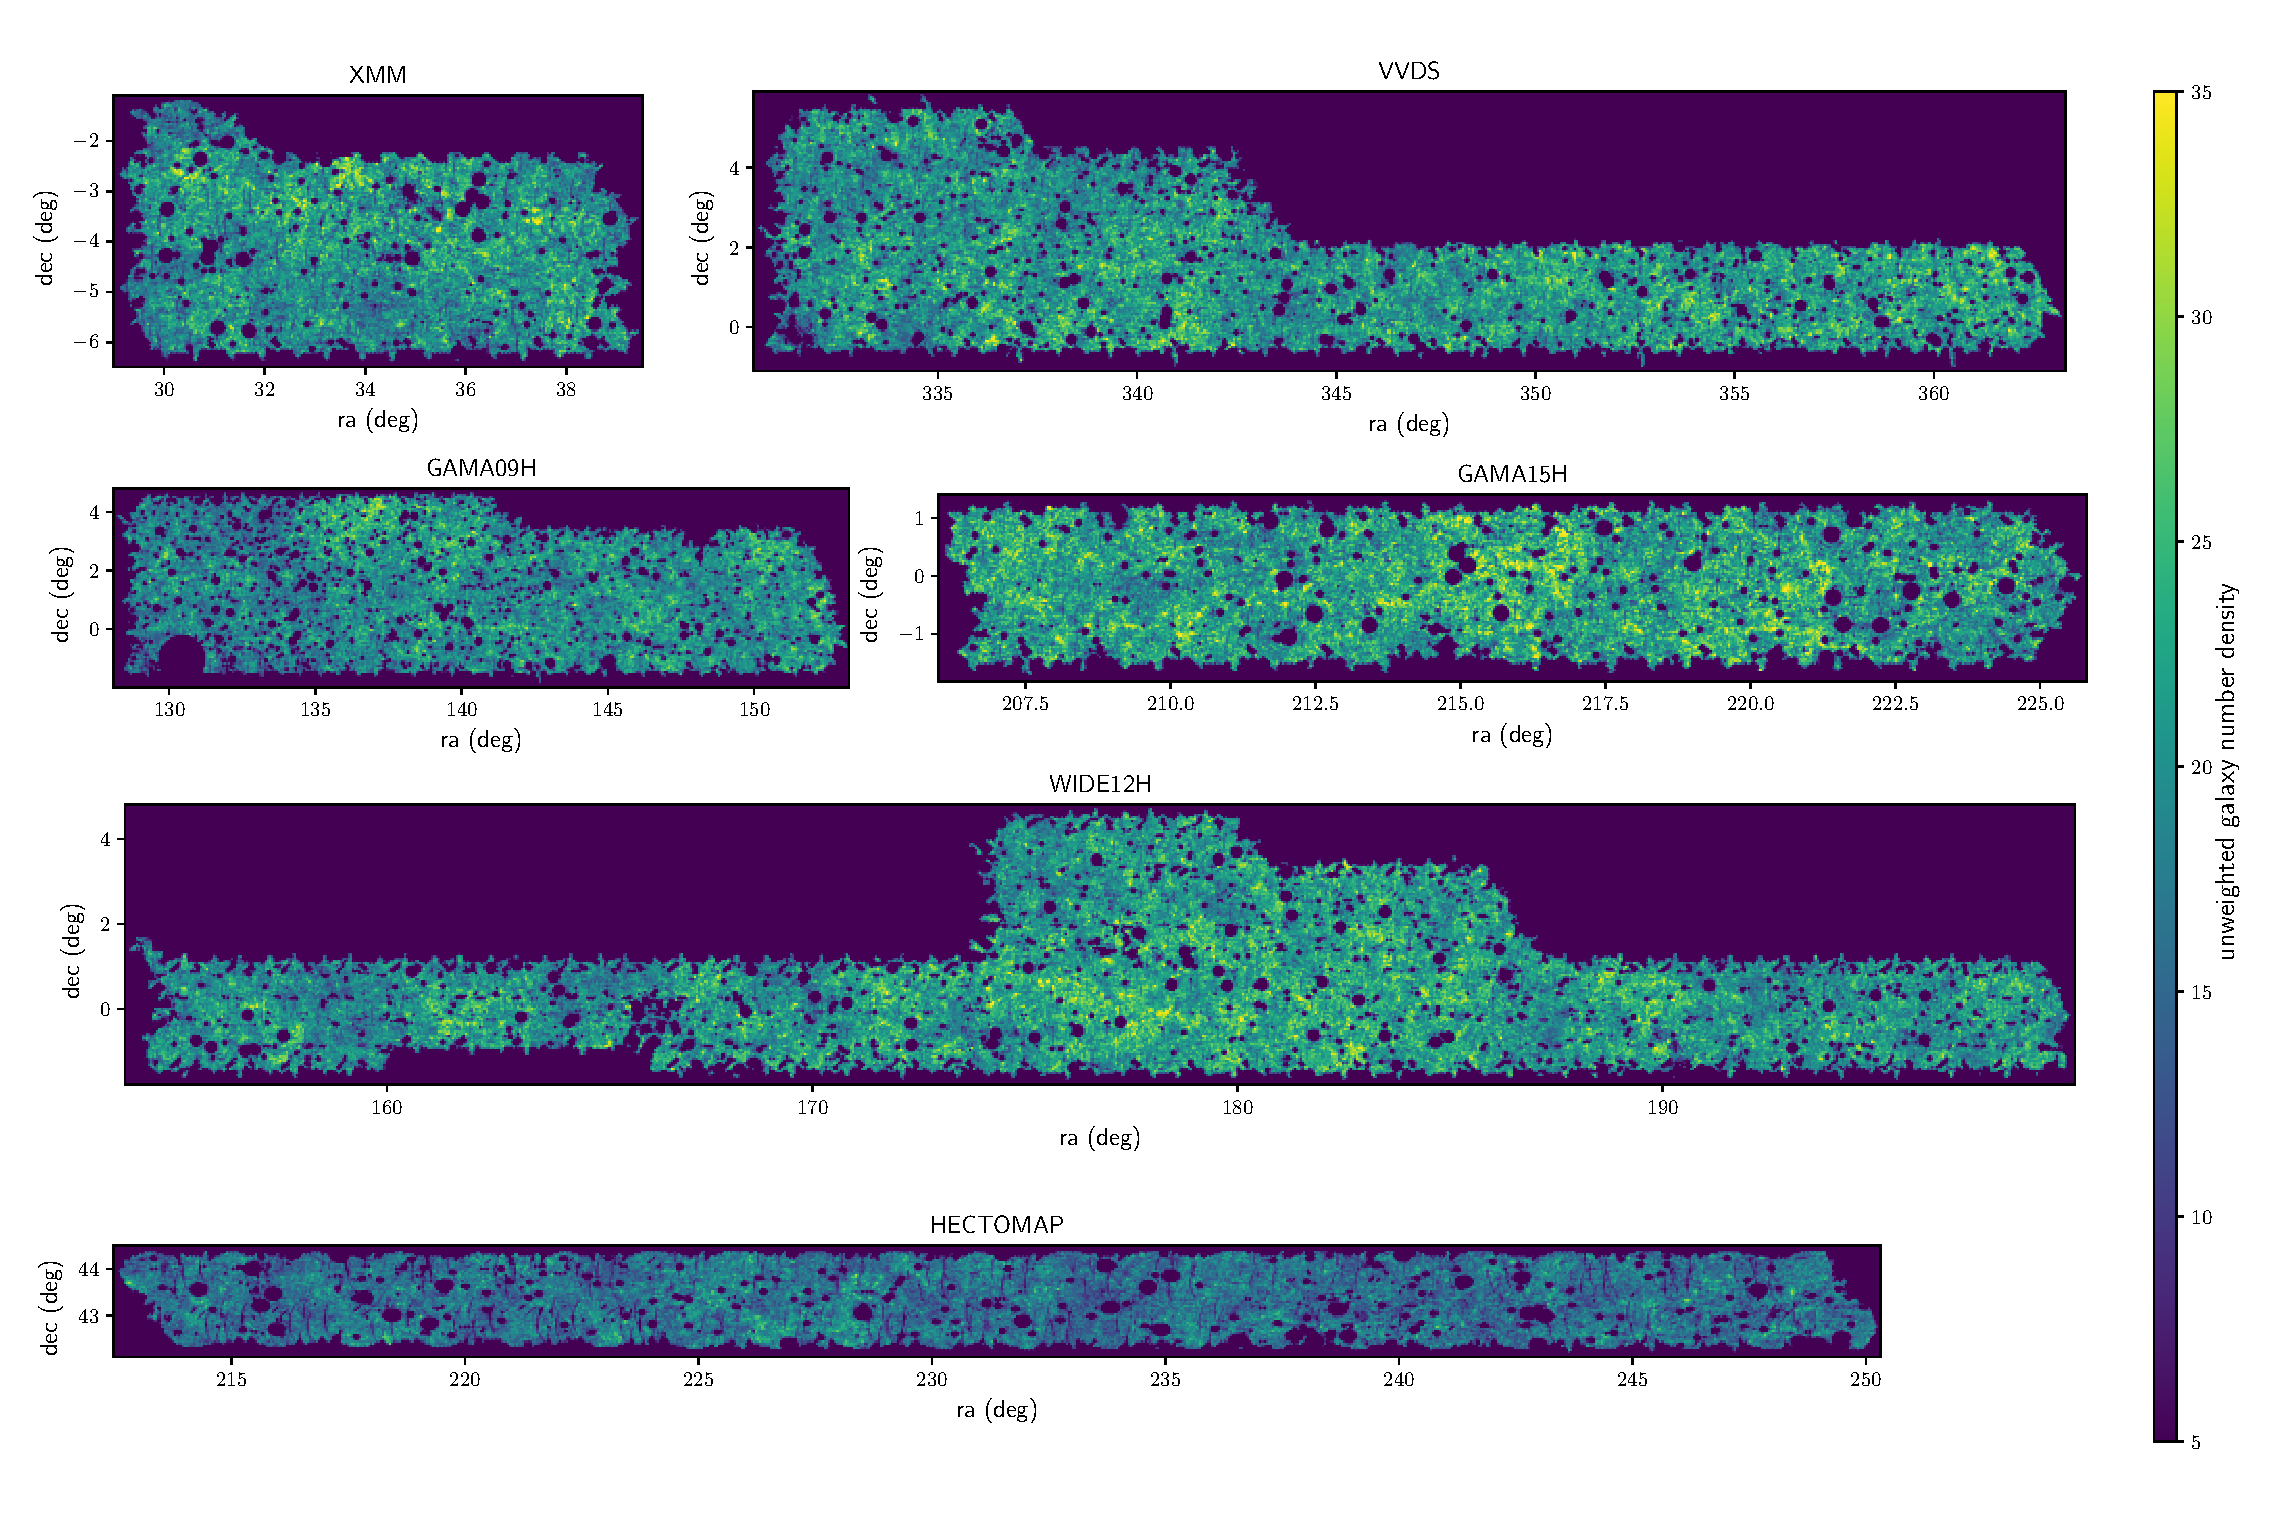
\includegraphics[width=0.9\textwidth]{densityMap.eps}
}
\caption{The galaxy number density map of the second year HSC shape catalog.
    The red scatters are the sampling positions of PSFs and noise variances.
    }
\end{figure*}

Our simulation is divided into $2500$ sub-samples and each sub-sample contains
$10^4$ postage-stamps with $64\times 64$ pixels. The pixel size is set to
$0.168$ arcesc. The noise property and PSF are the same for galaxies in one
sub-sample while they vary among different sub-samples. The HSC pipeline
reconstruct the PSF models and noise variances at any position of the coadd
images. We collect $2500$ noise variances and PSF models from a set of random
positions on the coadd images of HSC-WIDE layer within the footprint of the HSC
shape catalog.

Noise on the coadd images has spacial correlation due to the warping kernel
used to resample single exposures on the common pixel frame in the coadding
process. We sample the noise correlations from the blank pixels on the coadd
images. The sampled noise correlations, which are noisy at individual level,
are subsequently divided into eight groups and stacked in each group to create
eight different noise correlations with high signal to noise ratio.

Each sub-sample is assigned with a noise PSF model, noise variance and noise
correlation function. We then reweight each subsample to match the seeing
histograms and noise variance histograms of the simulation to the observation.
To note, the HSC WIDE layer is divided six observational fields (XMM, GAMA09H,
WIDE12H, GAMA15H, VVDS, HECTOMAP) and the reweighting is conducted for each
field. The seeing histograms and noise variance histograms of the observation
and simulation are shown in Figure \ref{fig:noiHist} and Figure
\ref{fig:fwhmHist}.

\begin{figure*}[ht!]
\centering{
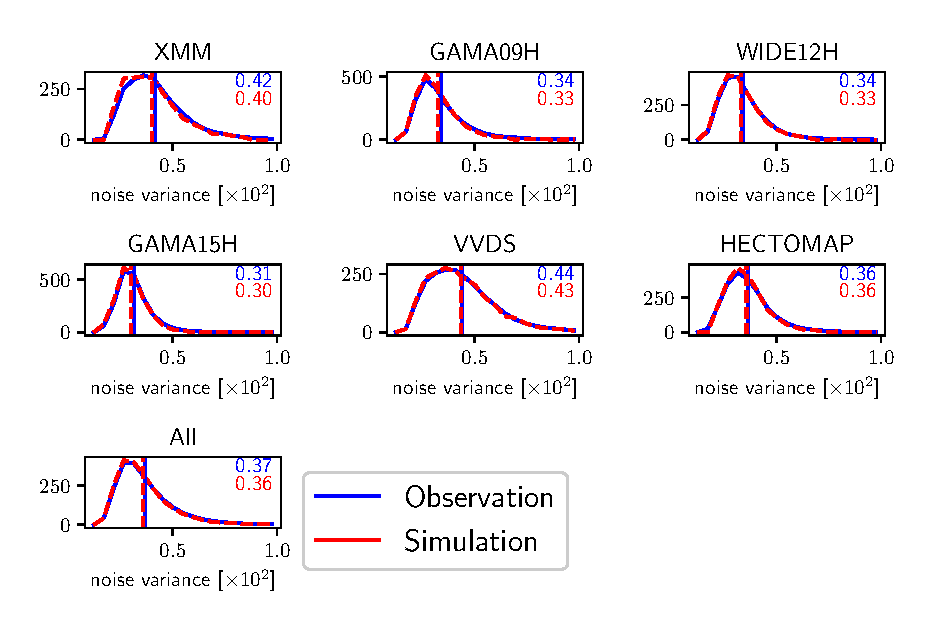
\includegraphics[width=0.9\textwidth]{noiVar_reCheck_recut.eps}
}
\caption{The first $6$ panels show the number histograms of noise variance for
    $6$ fields of the observation and the simulation. The last panel shows the
    histograms for the galaxies in all of the fields. The blue solid lines
    denote the observation and the red dashed lines denote the simulation. The
    blue texts show the average noise variance of the observation while the red
    texts show the average noise variance of the simulation.
    }
\label{fig:noiHist}
\end{figure*}

\begin{figure*}[ht!]
\centering{
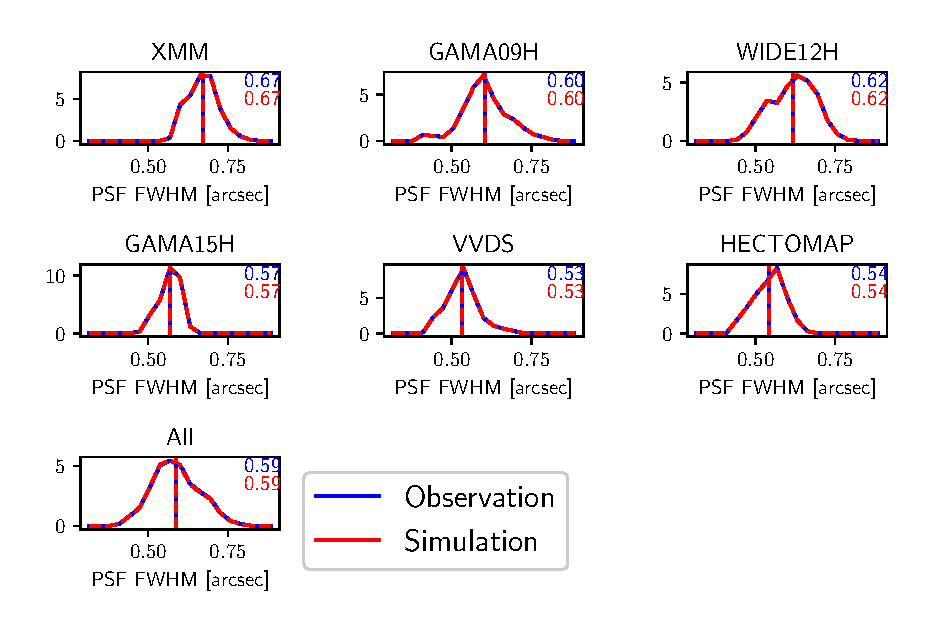
\includegraphics[width=0.9\textwidth]{psfFWHM_reCheck_recut.eps}
}
\caption{The first $6$ panels show the number histograms of noise variance for
    the $6$ fields of the observation and the simulation. The last panel shows
    the histograms for the galaxies in all of the fields. The blue solid lines
    denote the observation and the red dashed lines denote the simulation. The
    blue texts show the average FWHM of the observation while the red texts
    show the average FWHM of the simulation.
    }
\label{fig:fwhmHist}
\end{figure*}

\subsubsection{Galaxies}
We use the galaxy training sample created by \citet{HSC1-GREAT3Sim} as our
input galaxies. \citet{HSC1-GREAT3Sim} selects galaxies from the HSC WIDE-DEPTH
coadds \citep{HSC1-data} with CModel magnitude less than $25.2$.  Subsequently,
\citet{HSC1-GREAT3Sim} finds the centers of these selected galaxies on the
COSMOS-HST \citep{HST-ACSpipe} exposures and cuts out postage-stamps around
these positions. These positions are set to as the centers of the
postage-stamps and the postage sizes are required to be larger than $10.75$
arcsec to contain the galaxy light and structures of neighboring sources.

\citet{HSC1-GREAT3Sim} creates three training samples from three WIDE-DEPTH
coadds with different seeing values which are 0.5\arcsec, 0.7\arcsec and
1.0\arcsec. We use the training sample with the best seeing as our input galaxy
sample since it has the largest number of galaxies.

\galsim \citep{Galsim}, which is an open-source package for galaxy image
simulation, is used to simulate the HSC-like postage-stamps from the COSMOS HST
postage-stamp. The PSF is deconvolved from each input postage-stamp and then
the postage-stamp is convolved with an assigned HSC PSF model. The original
noise is whitened for each postage stamp then a noise with an assigned HSC
variance and HSC nosie correlation function is added to the postage-stamp.

\subsubsection{Image Processing} HSC pipeline is being developed to process the
data of HSC survey and will finally be applied to LSST survey. We use HSC
pipeline to detect galaxies from the simulated images and isolate blended
galaxies with HSC deblender to define a sample of sources. Subsequently, the
HSC pipeline is used to perform magnitude and shape measurements on the
detected sources.


\begin{figure*}[ht!]
\centering{
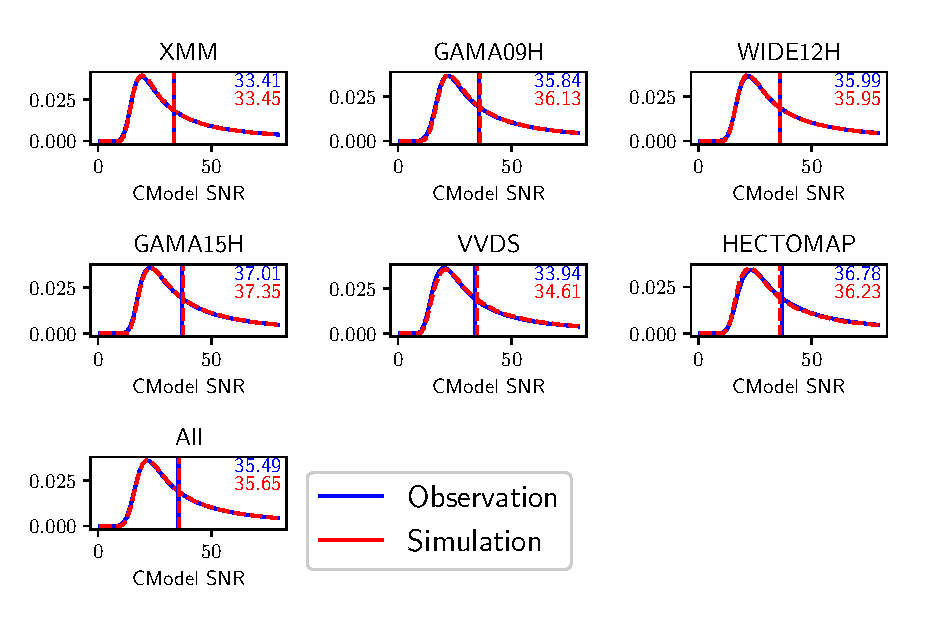
\includegraphics[width=0.9\textwidth]{snrDis_reCheck.eps}
}
\caption{The first 6 panels compare the number histograms of CModel SNR between
    the observation and the simulation for galaxies in 6 fields of the second
    year HSC shape catalog. The last panel shows the histograms for the
    galaxies in all of the fields. The blue solid lines are for the observation
    and the red dashed lines are for the simulation.
    }
\end{figure*}

\begin{figure*}[ht!]
\centering{
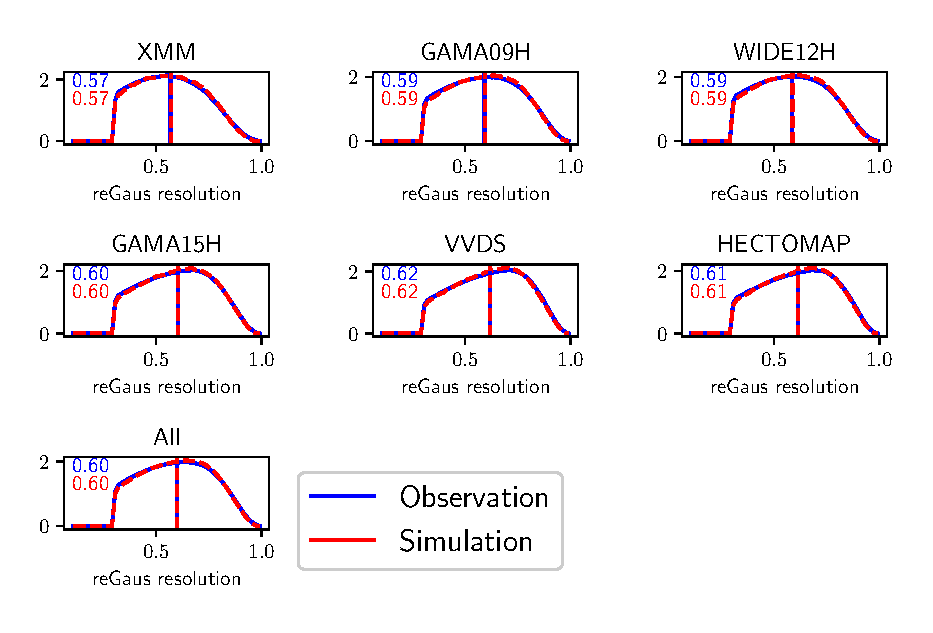
\includegraphics[width=0.9\textwidth]{resolutionDis_reCheck.eps}
}
\caption{The first 6 panels compare the number histograms of resolution between
    the observation and the simulation for galaxies in 6 fields of the second
    year HSC shape catalog. The last panel shows the histograms for the
    galaxies in all of the fields. The blue solid lines are for the observation
    and the red dashed lines are for the simulation.
    }
\end{figure*}


\begin{figure*}[ht!]
\centering{
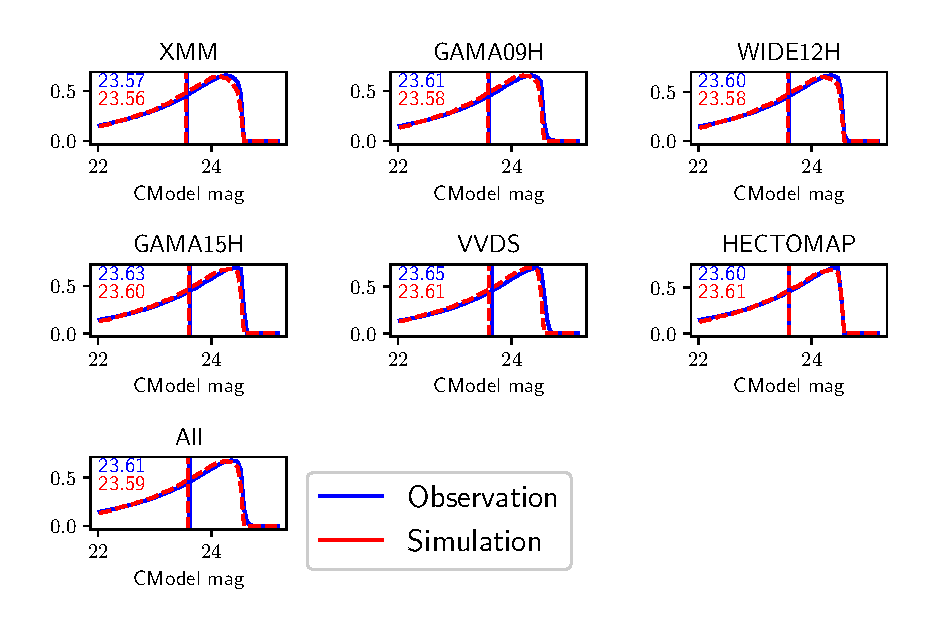
\includegraphics[width=0.9\textwidth]{magDis_reCheck.eps}
}
\caption{The first 6 panels compare the number histograms of CModel magnitude
    between the observation and the simulation for galaxies in 6 fields of the
    second year HSC shape catalog. The last panel shows the histograms for the
    galaxies in all of the fields. The blue solid lines are for the observation
    and the red dashed lines are for the simulation.
    }
\end{figure*}

\begin{figure*}[ht!]
\centering{
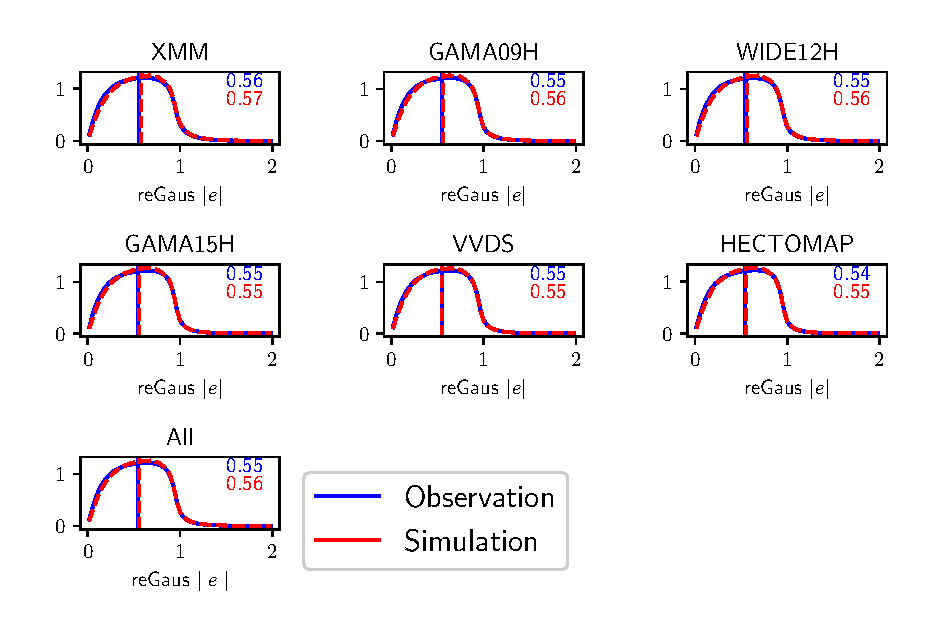
\includegraphics[width=0.9\textwidth]{absEDis_reCheck.eps}
}
\caption{The first 6 panels compare the number histograms of amplitude of
    ellipticity measured by re-gaussianization algorithm  between the
    observation and the simulation for galaxies in 6 fields of the second year
    HSC shape catalog. The last panel shows the histograms for the galaxies in
    all of the fields. The blue solid lines are for the observation and the red
    dashed lines are for the simulation.
    }
\end{figure*}


\subsection{Analysis}
\label{sec:Ana}
\begin{figure*}[ht!]
\centering{
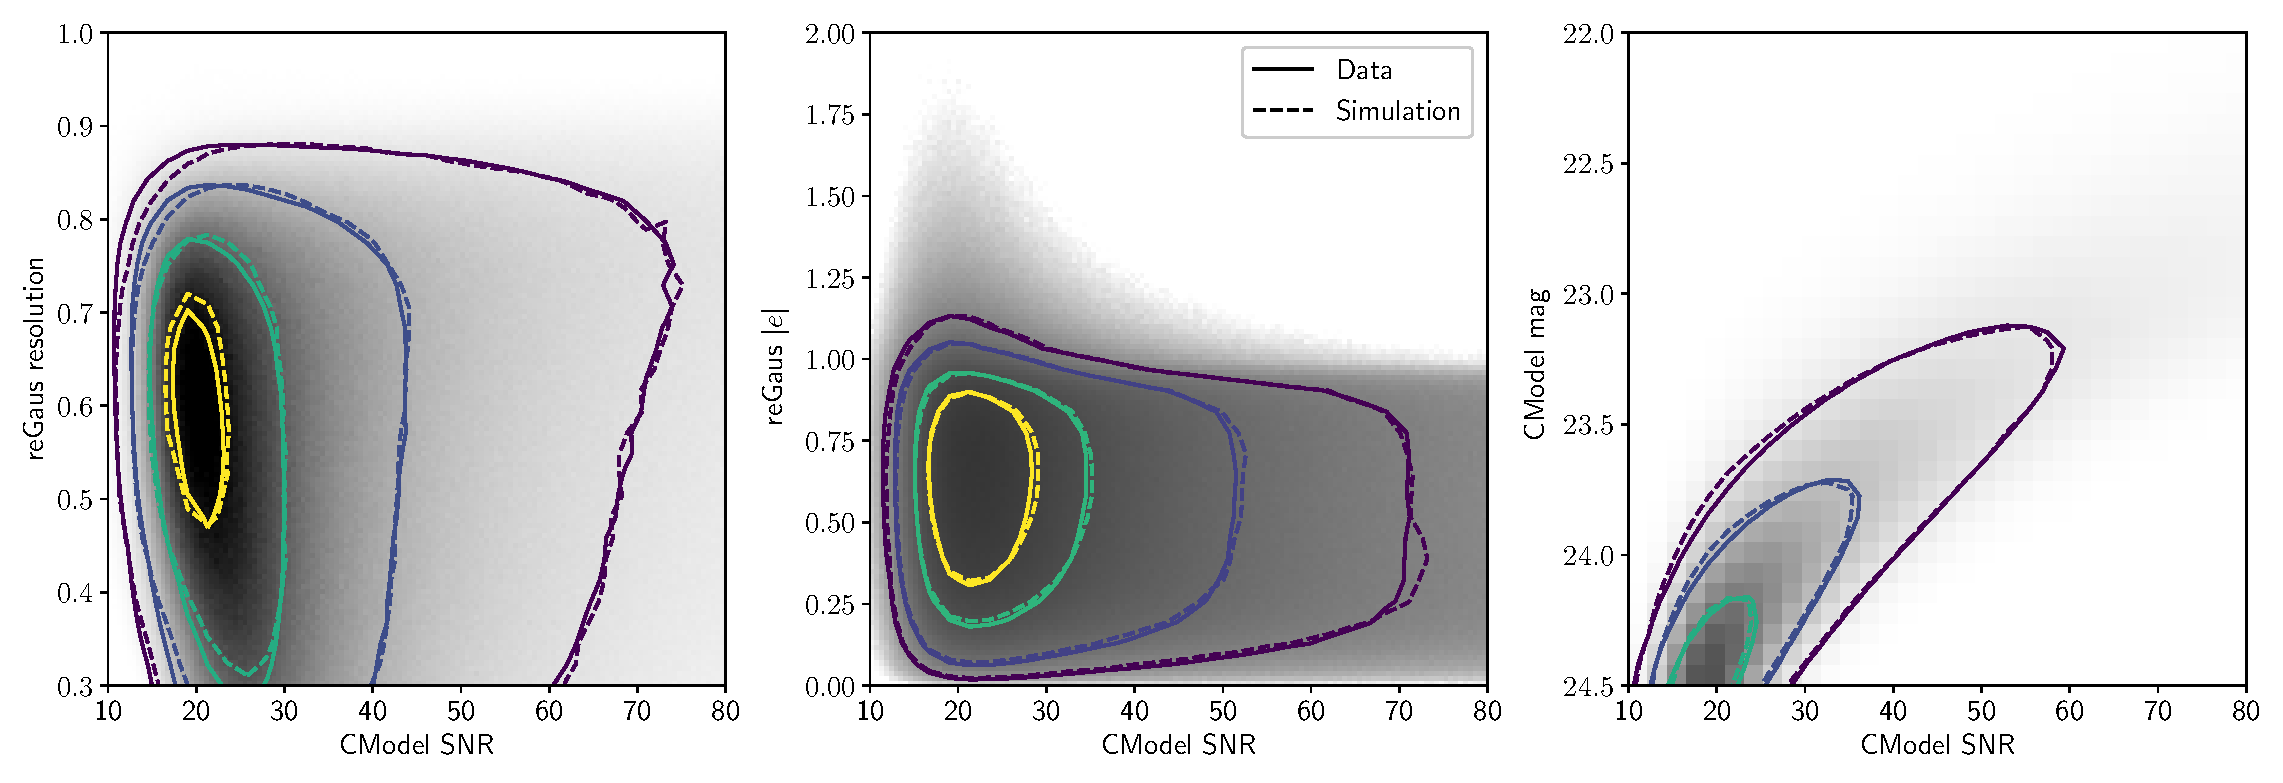
\includegraphics[width=0.9\textwidth]{galDis2D-final_reCheck.eps}
}
\caption{The $2$-D histograms of the simulation and the observation. The panels
    from left to right show the (SNR, resolution) histogram, (SNR, $\mid e
    \mid$) histogram and (SNR, CModel magnitude), respectively. The solid lines
    show the contours of the observation and the dashed lines show the contours
    of the simulation.
    }
\end{figure*}



\subsubsection{Optimization}
\begin{equation}
\sigma_e = 0.277 (\frac{\rm{SNR}}{20})^{-0.962} (\frac{\rm{res}}{0.5})^{-1.002}
\end{equation}


\begin{figure*}[ht!]
\centering{
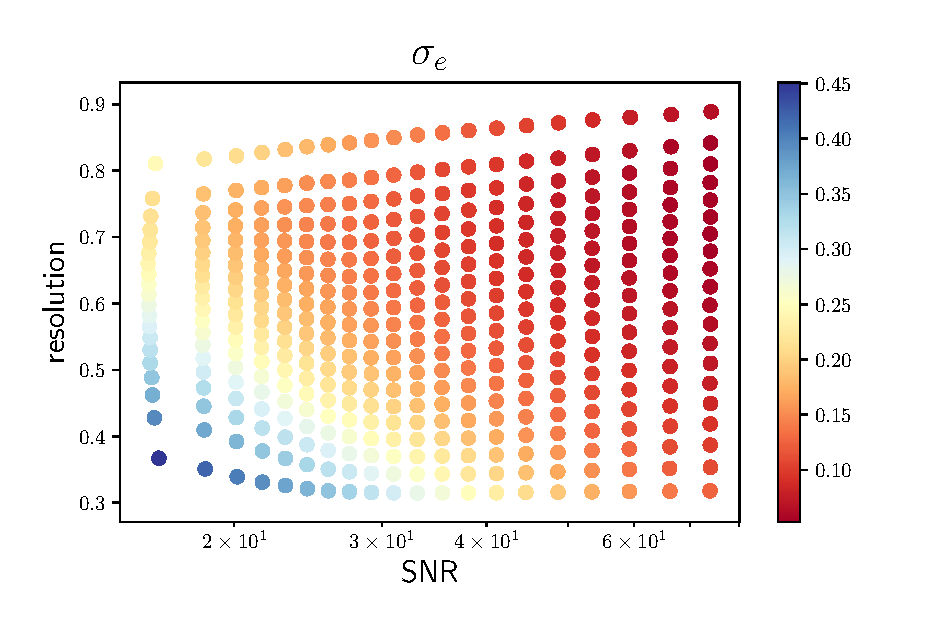
\includegraphics[width=0.45\textwidth]{sigmae_estimated.eps}
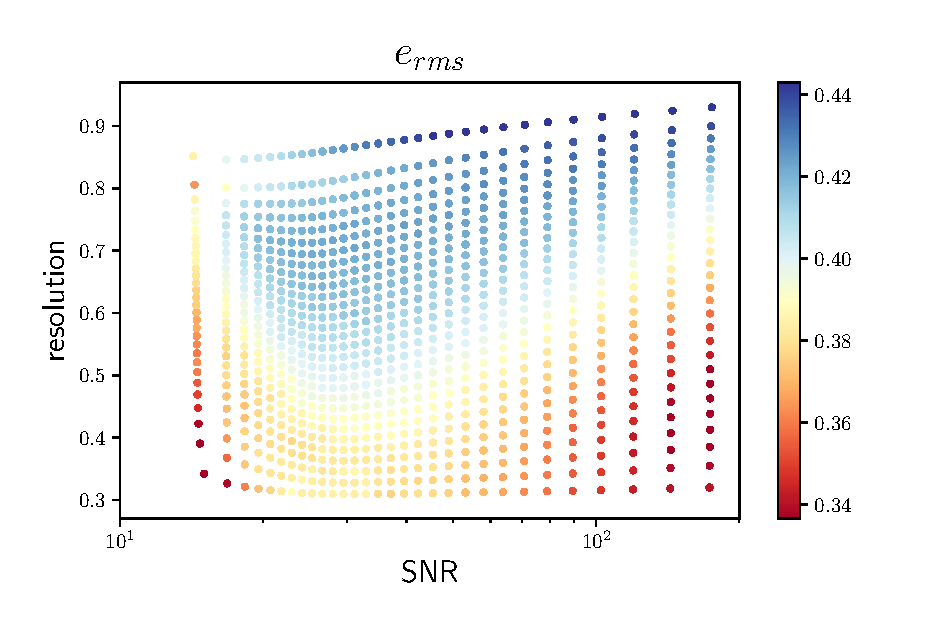
\includegraphics[width=0.45\textwidth]{intrinsicshape_2d.eps}
}
\caption{The left panel shows the shape measurement error per component
    ($\sigma_e$) estimated with the simulation in different (SNR, resolution)
    bins.  The right panel shows the intrinsic shape per component
    ($e_{\rm{RMS}}$) as function of (SNR, resolution).
    }
\end{figure*}

\subsubsection{Calibration Factors}

\subsubsection{Shear Bias}

\begin{figure*}[ht!]
\centering{
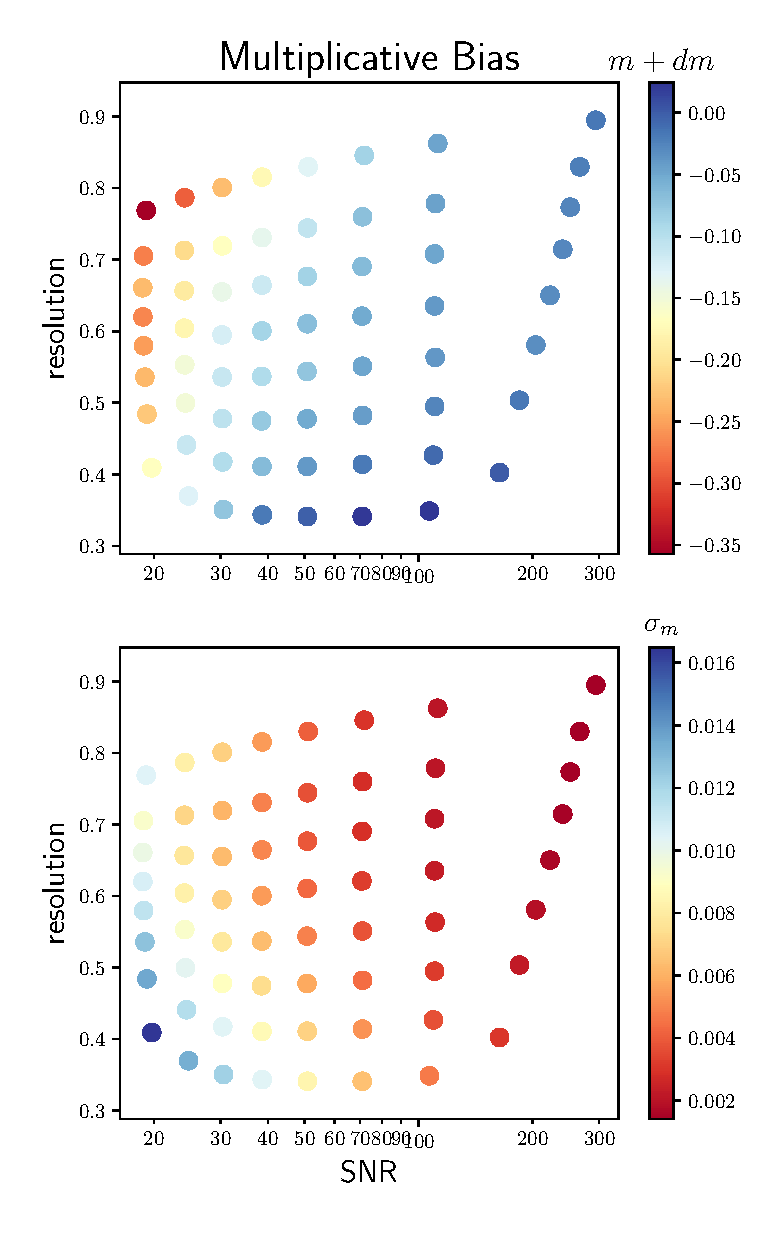
\includegraphics[width=0.45\textwidth]{shear_m_2d.eps}
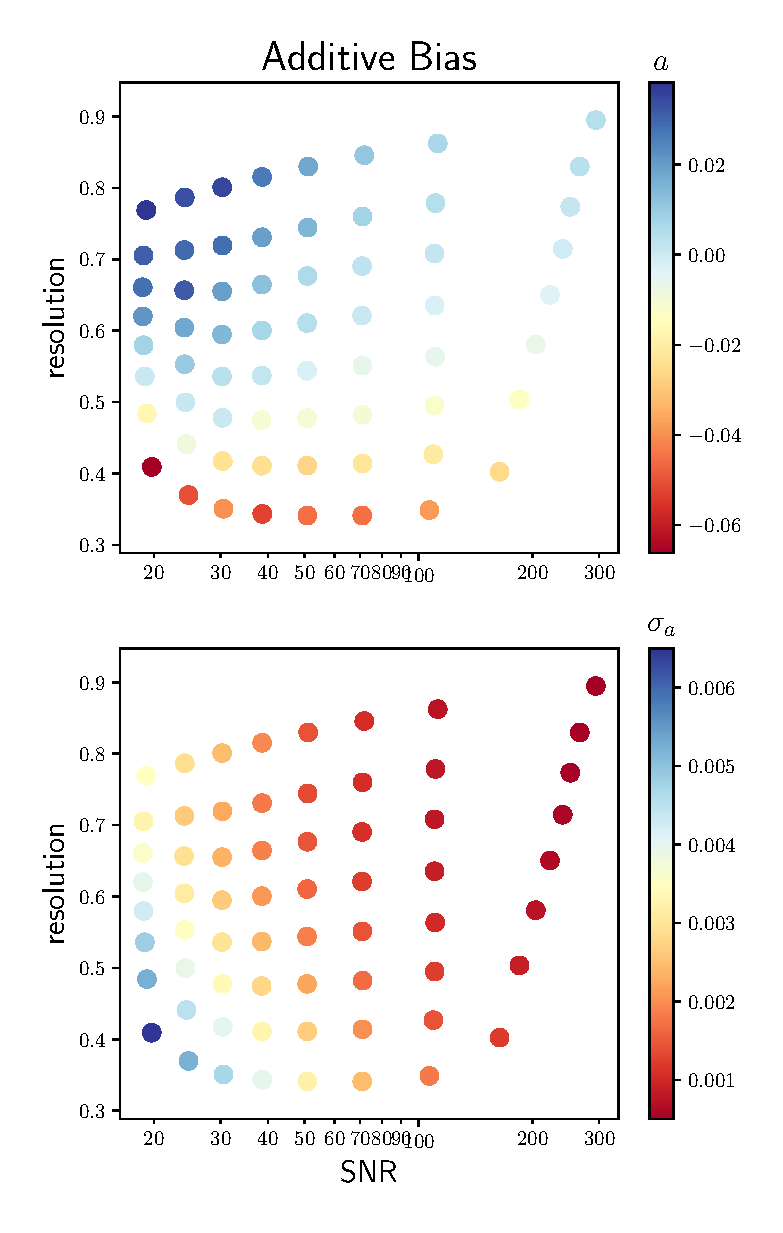
\includegraphics[width=0.45\textwidth]{shear_a_2d.eps}
}
\caption{The left panels show the multiplicative bias and the standard
    deviation of the multiplicative bias estimated in (SNR,resolution) bins
    with the simulation.  The right panels show the additive bias and the
    standard deviation of the additive bias estimated in (SNR,resolution) bins
    with the simulation.
    }
\end{figure*}

\begin{equation}
\hat{g}_{(1,2)}=\frac{\sum_i w_i e_{(1,2),i} }{2\res (1+\hat{m}) \sum_i w_i}-\frac{\hat{c}_{(1,2)}}{1+\hat{m}}
\end{equation}


\begin{equation}
m + \rm{const.} \propto (\frac{\rm{res}}{0.5})^{1.66}(\frac{\rm{snr}}{20})^{-1.24}
\end{equation}
\begin{equation}
a \propto (\rm{res}-0.61)(\frac{\rm{snr}}{20})^{-0.94}
\end{equation}

\subsubsection{Weight Bias}
\begin{figure*}[ht!]
\centering{
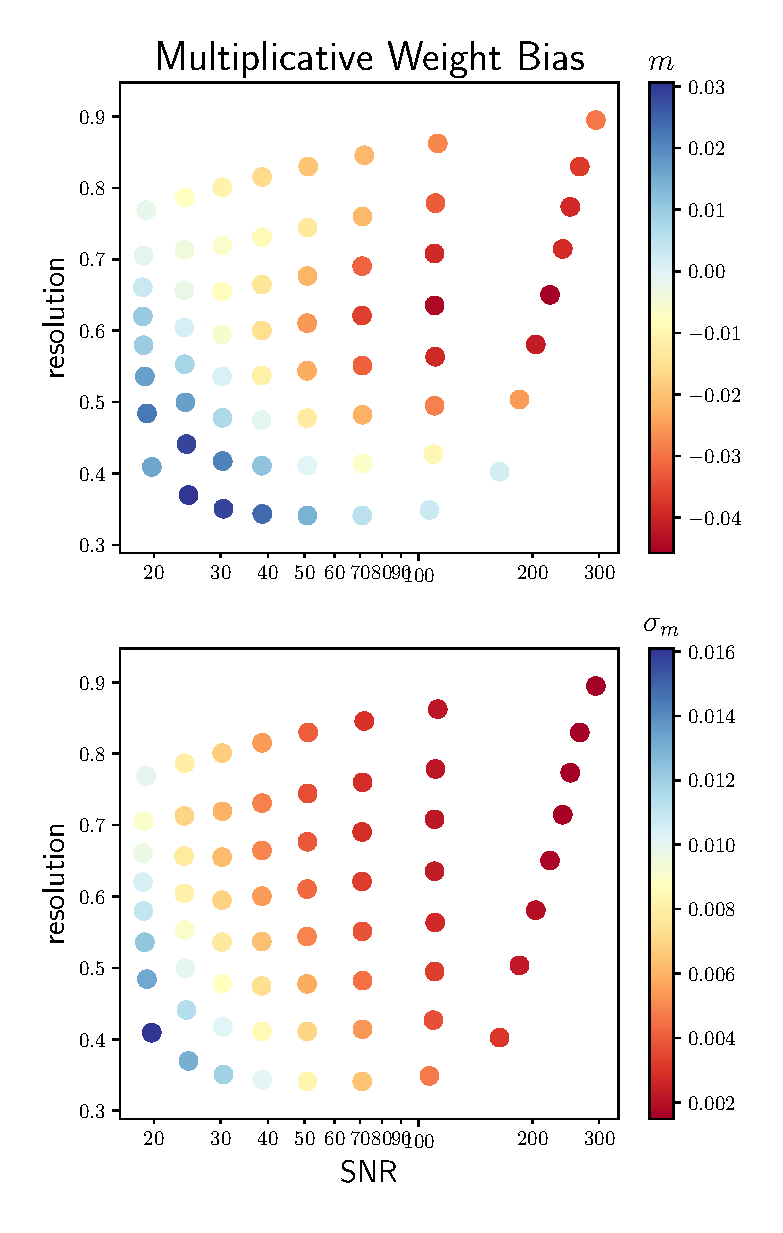
\includegraphics[width=0.45\textwidth]{weightBias_m_2d.eps}
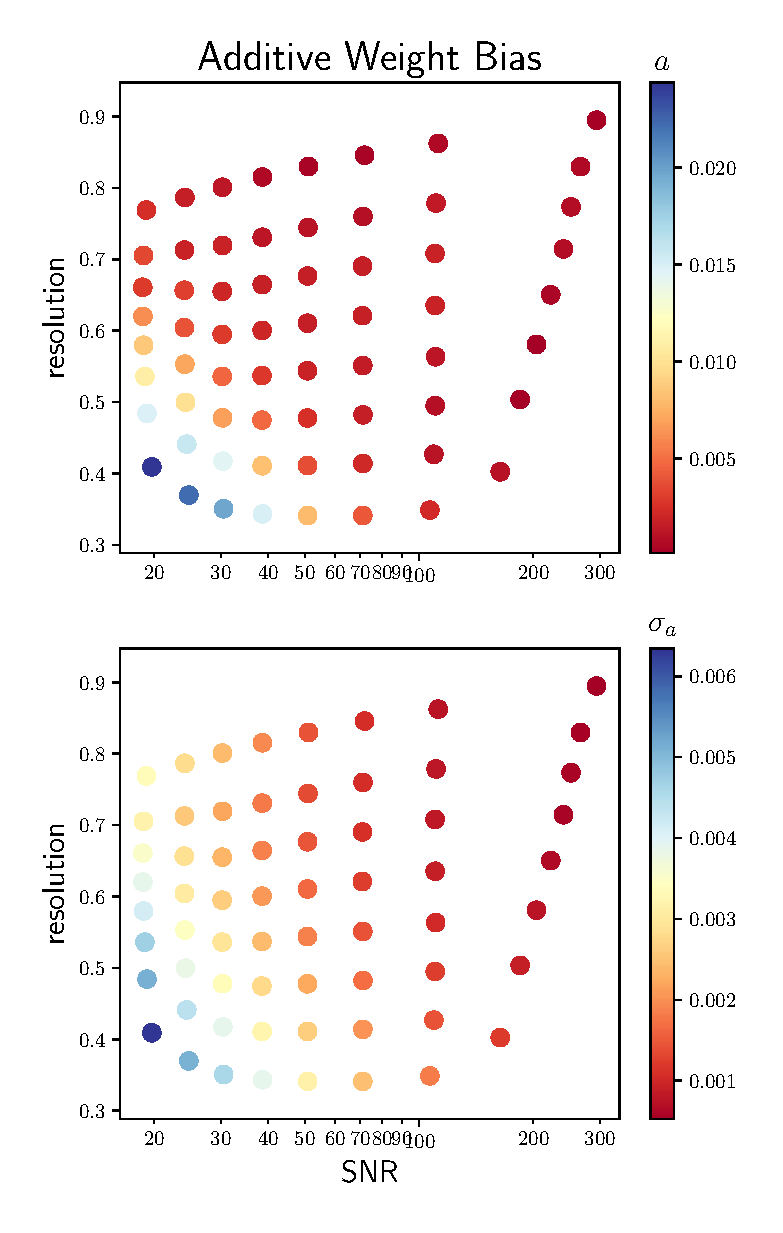
\includegraphics[width=0.45\textwidth]{weightBias_a_2d.eps}
}
\caption{The left panels show the multiplicative weight bias and the standard
    deviation of the multiplicative bias estimated in (SNR,resolution) bins
    with the simulation.  The right panels show the additive weight bias and
    the standard deviation of the additive bias estimated in (SNR,resolution)
    bins with the simulation.
    }
\end{figure*}

\subsubsection{Redshift Dependence}
\begin{figure*}[ht!]
\centering{
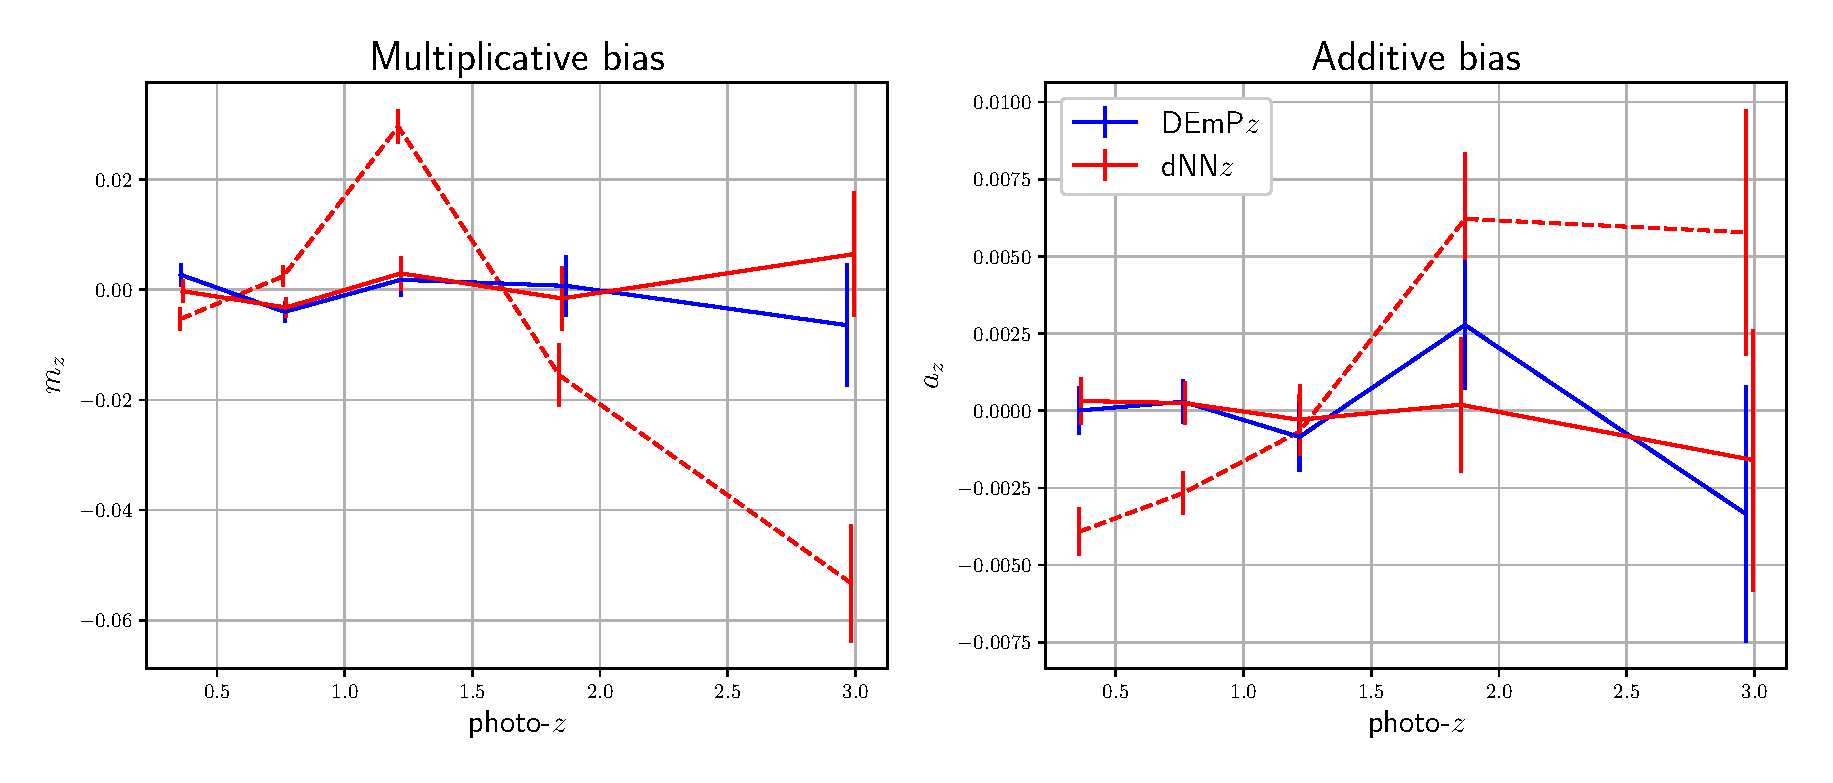
\includegraphics[width=0.9\textwidth]{calibration_residual_redshfits.eps}
}
\caption{The left panel shows the multiplicative bias residual estimated in
    photo-$z$ bins.  The right panel shows the additive bias residual estimated
    in photo-$z$ bins.  The red lines are for DEmPz, and the blue lines are for
    dNNz.  The dashed lines are the results before calibrating the redshift
    dependent bias, whereas the solid lines are the results after calibrating
    the redshift dependent bias using dNNz.
    }
\end{figure*}

\subsection{Sanity Test}
\subsubsection{Modeled Observables}
\begin{figure*}[ht!]
\centering{
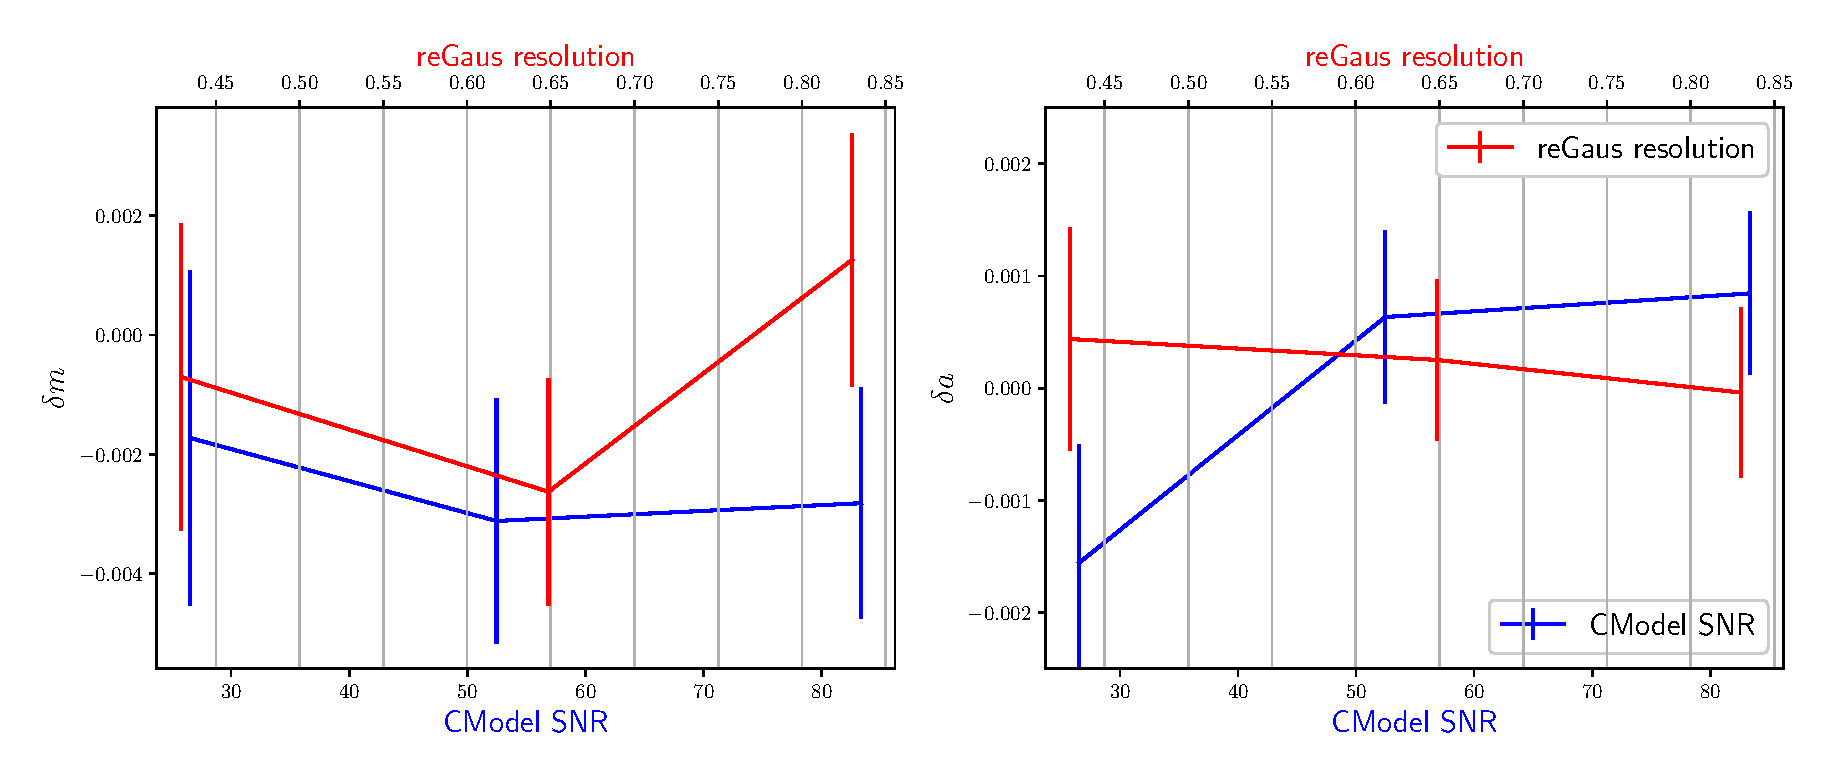
\includegraphics[width=0.9\textwidth]{calibration_residual_modeled.eps}
}
\caption{The dependence of calibration residuals the modeled properties.
        }
\end{figure*}

\subsubsection{Marginalized Observables}
\begin{figure*}[ht!]
\centering{
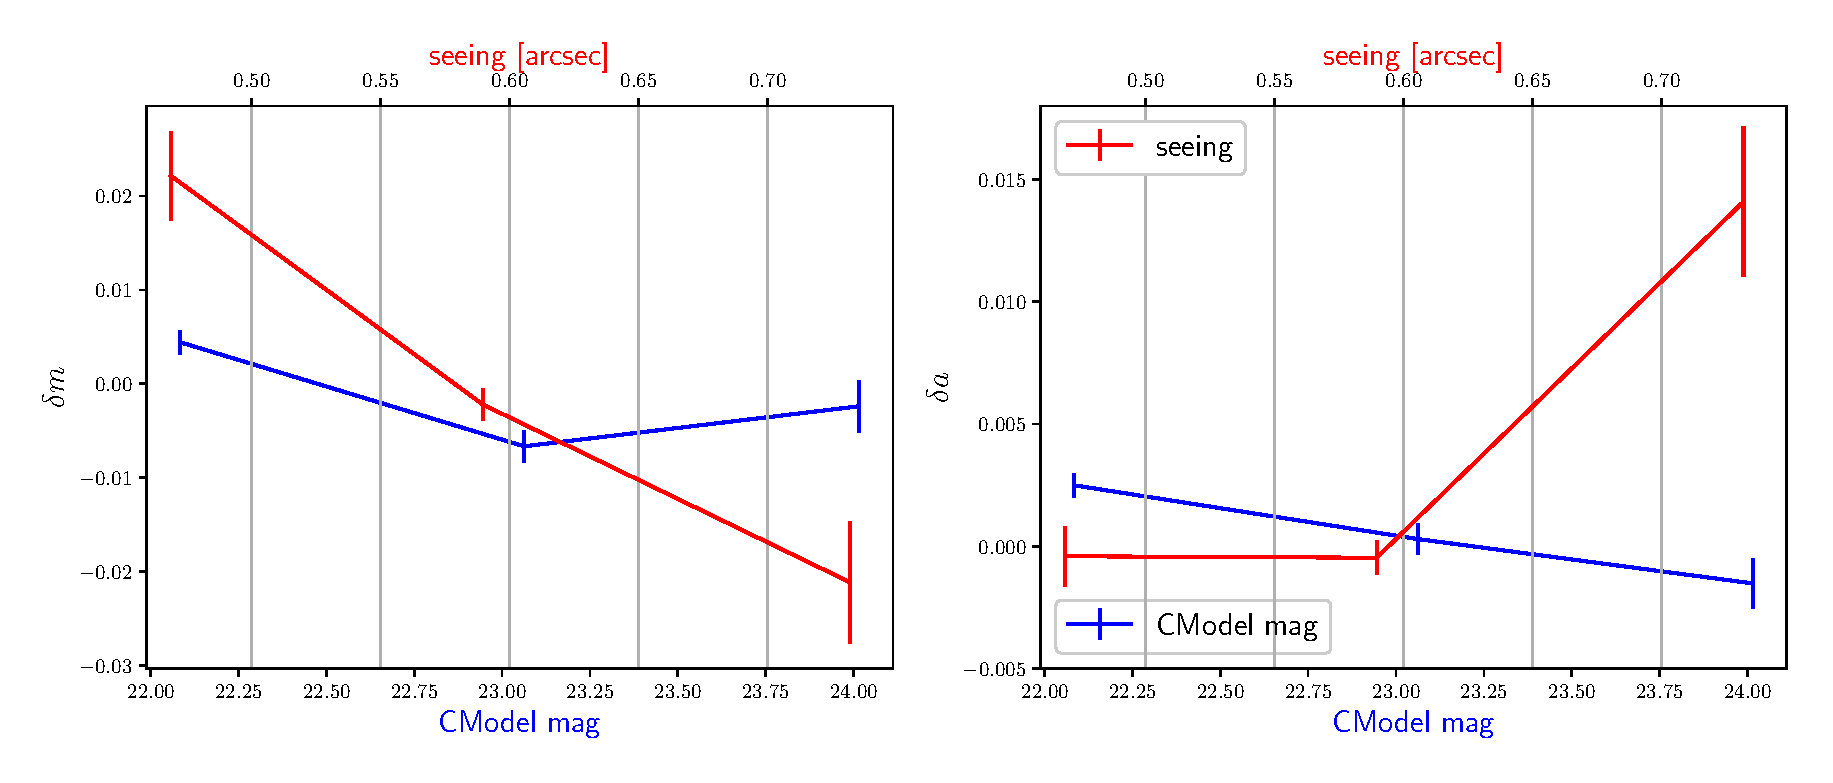
\includegraphics[width=0.9\textwidth]{calibration_residual_marginalized.eps}
}
\caption{The dependence of calibration residuals the marginalized properties.
        }
\end{figure*}

\subsection{Selection Bias}

\begin{figure*}[ht!]
\centering{
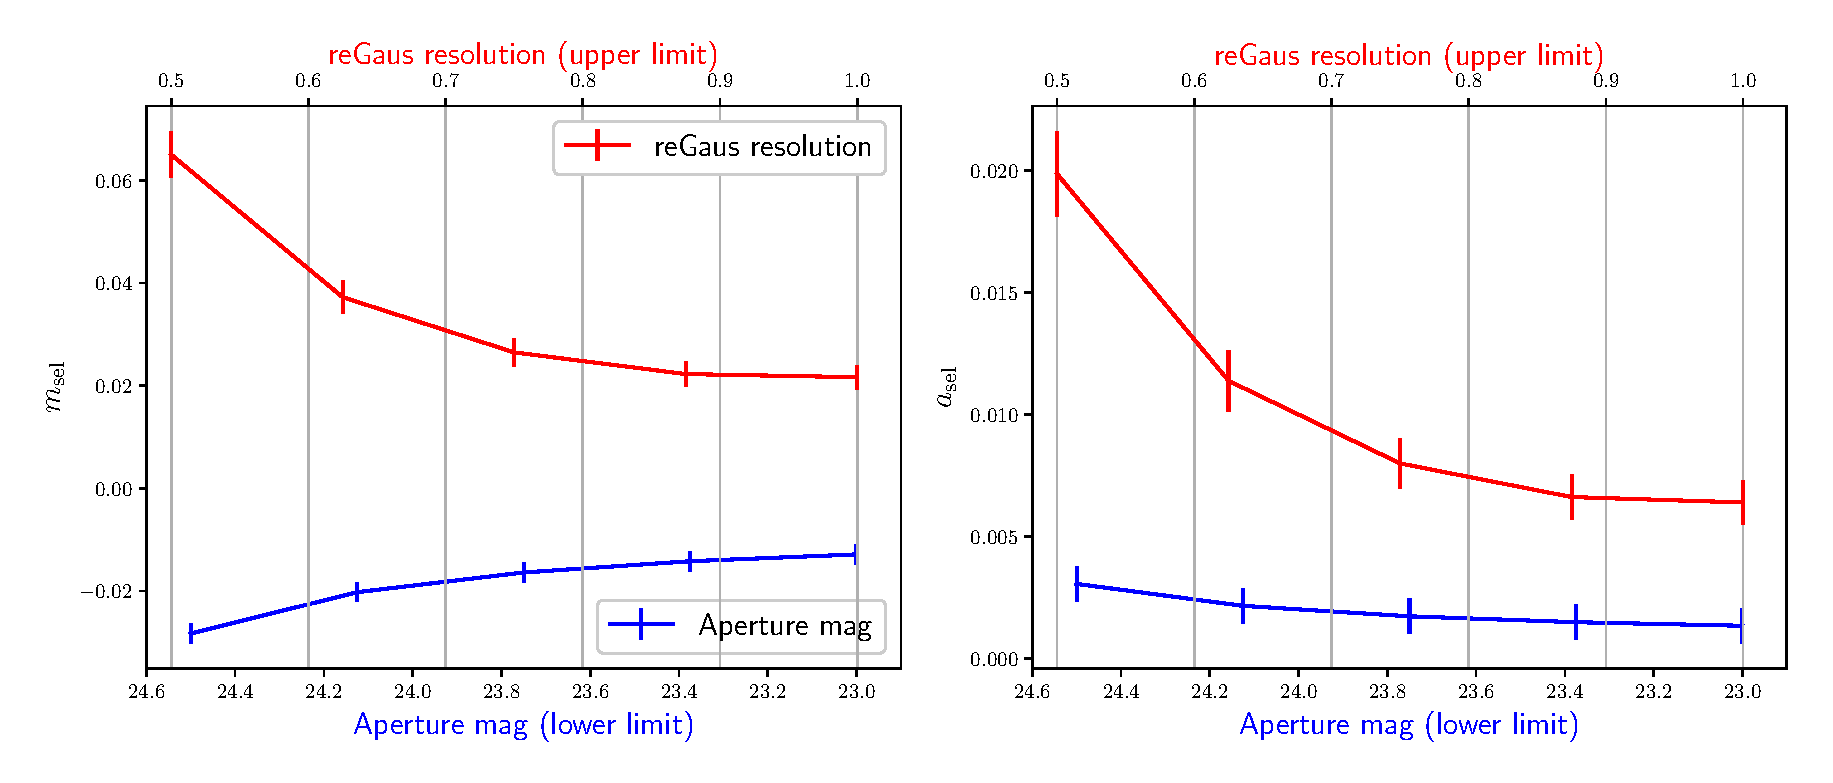
\includegraphics[width=0.9\textwidth]{selBias_res_magA10.eps}
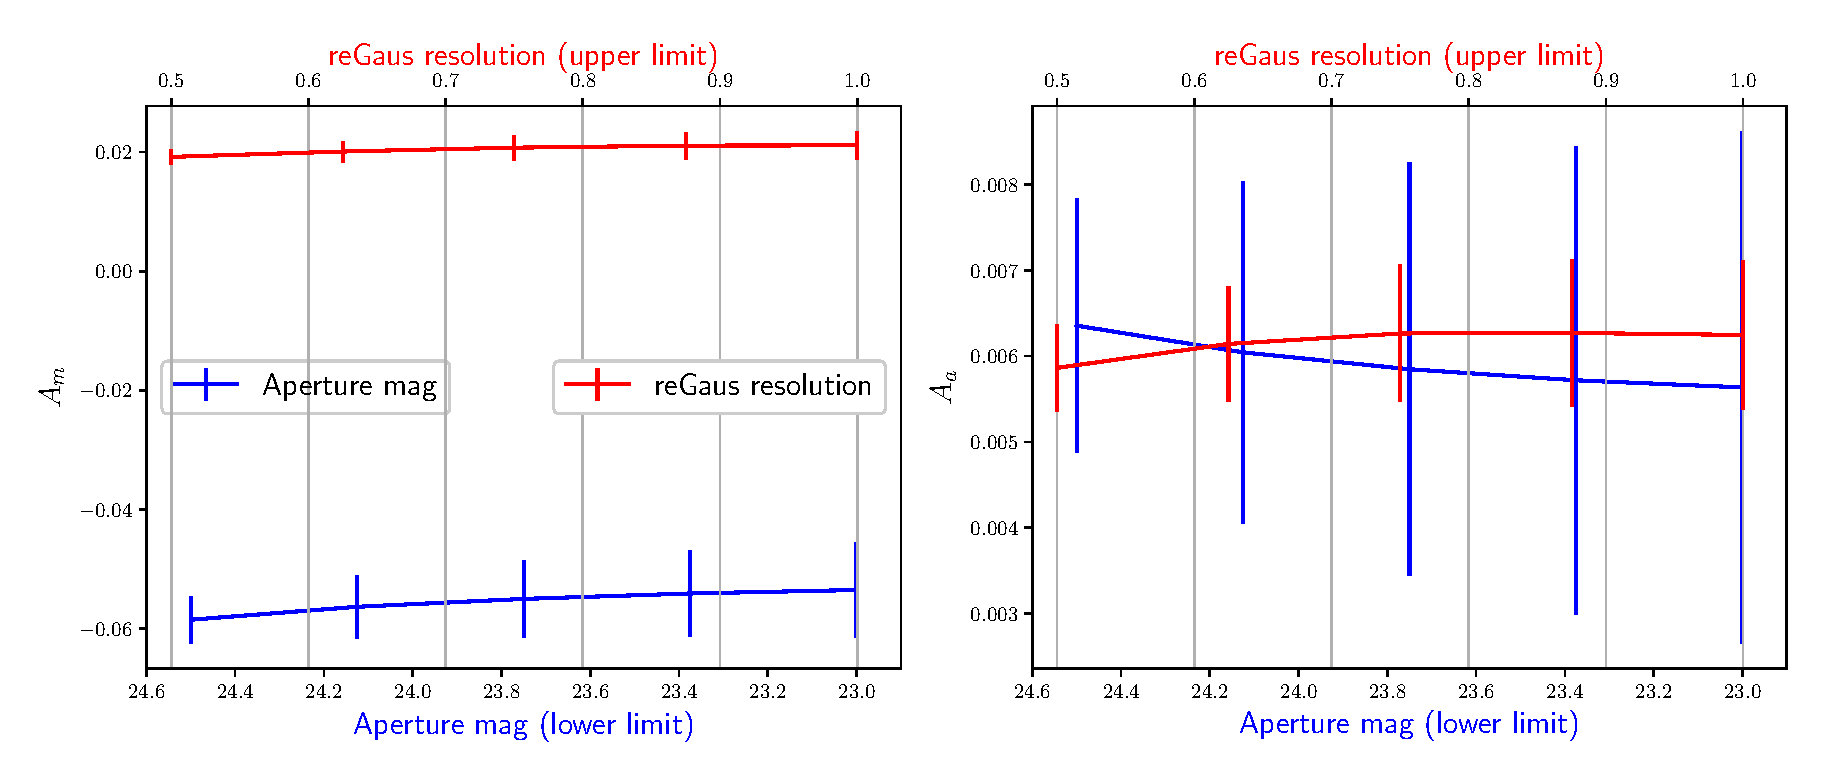
\includegraphics[width=0.9\textwidth]{selBias_ratio_res_magA10.eps}
}
\caption{
        }
\end{figure*}

\begin{table}
\centering
  \begin{tabular}{ll} \hline
    Output properties & Meaning \\ \hline
\multicolumn{2}{c}{Optimization} \\ \hline
\texttt{i$\_$hsmshaperegauss$\_$derived$\_$sigma$\_$e}& Error due to photon noise \\ \hline
\texttt{i$\_$hsmshaperegauss$\_$derived$\_$rms$\_$e}  & Shape noise\\ \hline
\texttt{i$\_$hsmshaperegauss$\_$derived$\_$weight}    & weak lensing shape weight\\ \hline
\multicolumn{2}{c}{Calibration} \\ \hline
\texttt{i$\_$hsmshaperegauss$\_$derived$\_$shear$\_$bias$\_$m} & multiplicative bias\\ \hline
\texttt{i$\_$hsmshaperegauss$\_$derived$\_$shear$\_$bias$\_$c1}& the first component of additive bias\\ \hline
\texttt{i$\_$hsmshaperegauss$\_$derived$\_$shear$\_$bias$\_$c2}& the second component of additive bias\\ \hline
\hline
  \end{tabular}
  \caption{}
\end{table}

\section{Calibration}

\section{Blinding}
\label{sec:blind}

\section{Null Tests (galaxy shape tests)}
\label{sec:nullTest}
\begin{enumerate}
    \item shear around random points
    \item shear around stars
    \item x shear around CMASS galaxies
    \item g1 vs (cmodel SN, cmodel, resolution, PSF FWHM): Ask Oguri-san to compute this again with the updated catalog
    \item star-star correlations, star-galaxy correlations, and shear-shear correlations: Ask Hamana-san to compute this again with the updated catalog
    \item mass maps
\end{enumerate}

\section{Other tests}
\subsection{contamination by stars}
Just repeat the same test with the S19A catalog.

\section{Summary}
\label{sec:summary}


\bibliographystyle{apj}
\bibliography{citation}


\appendix
\section*{Galaxy Selection}
\label{App:select}
\begin{table*}
  \begin{tabular}{ll} \hline
    Cut & Meaning \\ \hline
\multicolumn{2}{c}{Basic flag cuts} \\ \hline
\texttt{i$\_$detect$\_$isprimary} $==$ True & Identify unique detections only \\ \hline
\texttt{i$\_$deblend$\_$skipped} $==$ False & Deblender skipped this group of objects \\ \hline
\hmrv{\texttt{i$\_$sdsscentroid$\_$flag} $==$ False} & \hmrv{centroid.sdss measurement failed} \\ \hline
\texttt{i$\_$pixelflags$\_$edge} $==$ False & Object too close to image boundary for reliable measurements \\ \hline
\texttt{i$\_$pixelflags$\_$interpolatedcenter} $==$ False & A pixel flagged as interpolated is
close to object center \\ \hline
\texttt{i$\_$pixelflags$\_$saturatedcenter} $==$ False & A pixel flagged as saturated is
close to object center \\ \hline
\texttt{i$\_$pixelflags$\_$crcenter}$==$ False & A pixel flagged as a cosmic ray hit is
close to object center \\ \hline
\texttt{i$\_$pixelflags$\_$bad}$==$ False & A pixel flagged as otherwise bad is
close to object center \\ \hline
\texttt{i$\_$pixelflags$\_$suspectcenter} $==$ False & A pixel flagged as near saturation is
close to object center \\ \hline
\hmrv{\texttt{i$\_$pixelflags$\_$clipped} $==$ False} & \hmrv{Flagged as source footprint includes clipped pixels} \\ \hline
\texttt{i$\_$hsmshaperegauss$\_$flag} $==$ False & Error code returned by shape measurement
code \\ \hline
\texttt{i$\_$hsmshaperegauss$\_$sigma} $!=$ NaN & Shape measurement uncertainty should not be
  NaN \\ \hline
\texttt{i$\_$extendedness$\_$value} $!= 0$ & Extended object \\ \hline
\multicolumn{2}{c}{Cuts on object properties} \\ \hline
\texttt{i$\_$cmodel$\_$flux}/\texttt{i$\_$cmodel$\_$fluxerr} $\ge 10$ & Galaxy has high enough $S/N$ in
$i$ band\\
\hline
\texttt{i$\_$hsmshaperegauss$\_$resolution} $\ge 0.3$ & Galaxy is sufficiently resolved \\ \hline
(\texttt{i$\_$hsmshaperegauss$\_$e1}$^2 + $\texttt{i$\_$hsmshaperegauss$\_$e2}$^2)^{1/2} < 2$ & Total
\rmrv{distortion} cut \\ \hline
$0\le $\texttt{i$\_$hsmshaperegauss$\_$sigma}  $\le 0.4$ & Estimated shape measurement error is
reasonable \\ \hline
\texttt{i$\_$cmodel$\_$mag} $-$ \texttt{a$\_$i} $\le 24.5$ & Magnitude cut \\ \hline
\texttt{i$\_$apertureflux$\_$10$\_$mag} $\le 25.5$ & Aperture magnitude cut \\ \hline
\texttt{i$\_$blendedness$\_$abs} $< 10^{-0.38}$ & Avoid spurious detections and those
contaminated by blends \\ \hline
\multicolumn{2}{c}{Require that at least two of the following four cuts be passed (not all)} \\ \hline
\texttt{g$\_$cmodel$\_$flux}/\texttt{g$\_$cmodel$\_$fluxerr} $\ge 5$ & Galaxy has high enough $S/N$ in
$g$ band\\
\hline
\texttt{r$\_$cmodel$\_$flux}/\texttt{r$\_$cmodel$\_$fluxerr} $\ge 5$ & Galaxy has high enough $S/N$ in
$r$ band\\
\hline
\texttt{z$\_$cmodel$\_$flux}/\texttt{z$\_$cmodel$\_$fluxerr} $\ge 5$ & Galaxy has high enough $S/N$ in
$z$ band\\
\hline
\texttt{y$\_$cmodel$\_$flux}/\texttt{y$\_$cmodel$\_$fluxerr} $\ge 5$ & Galaxy has high enough $S/N$ in
$y$ band\\
\hline
  \end{tabular}
  \caption{}
\end{table*}

\end{document}

\section*{The redshift dependence of intrinsic shape}
\begin{figure*}[ht!]
\centering{
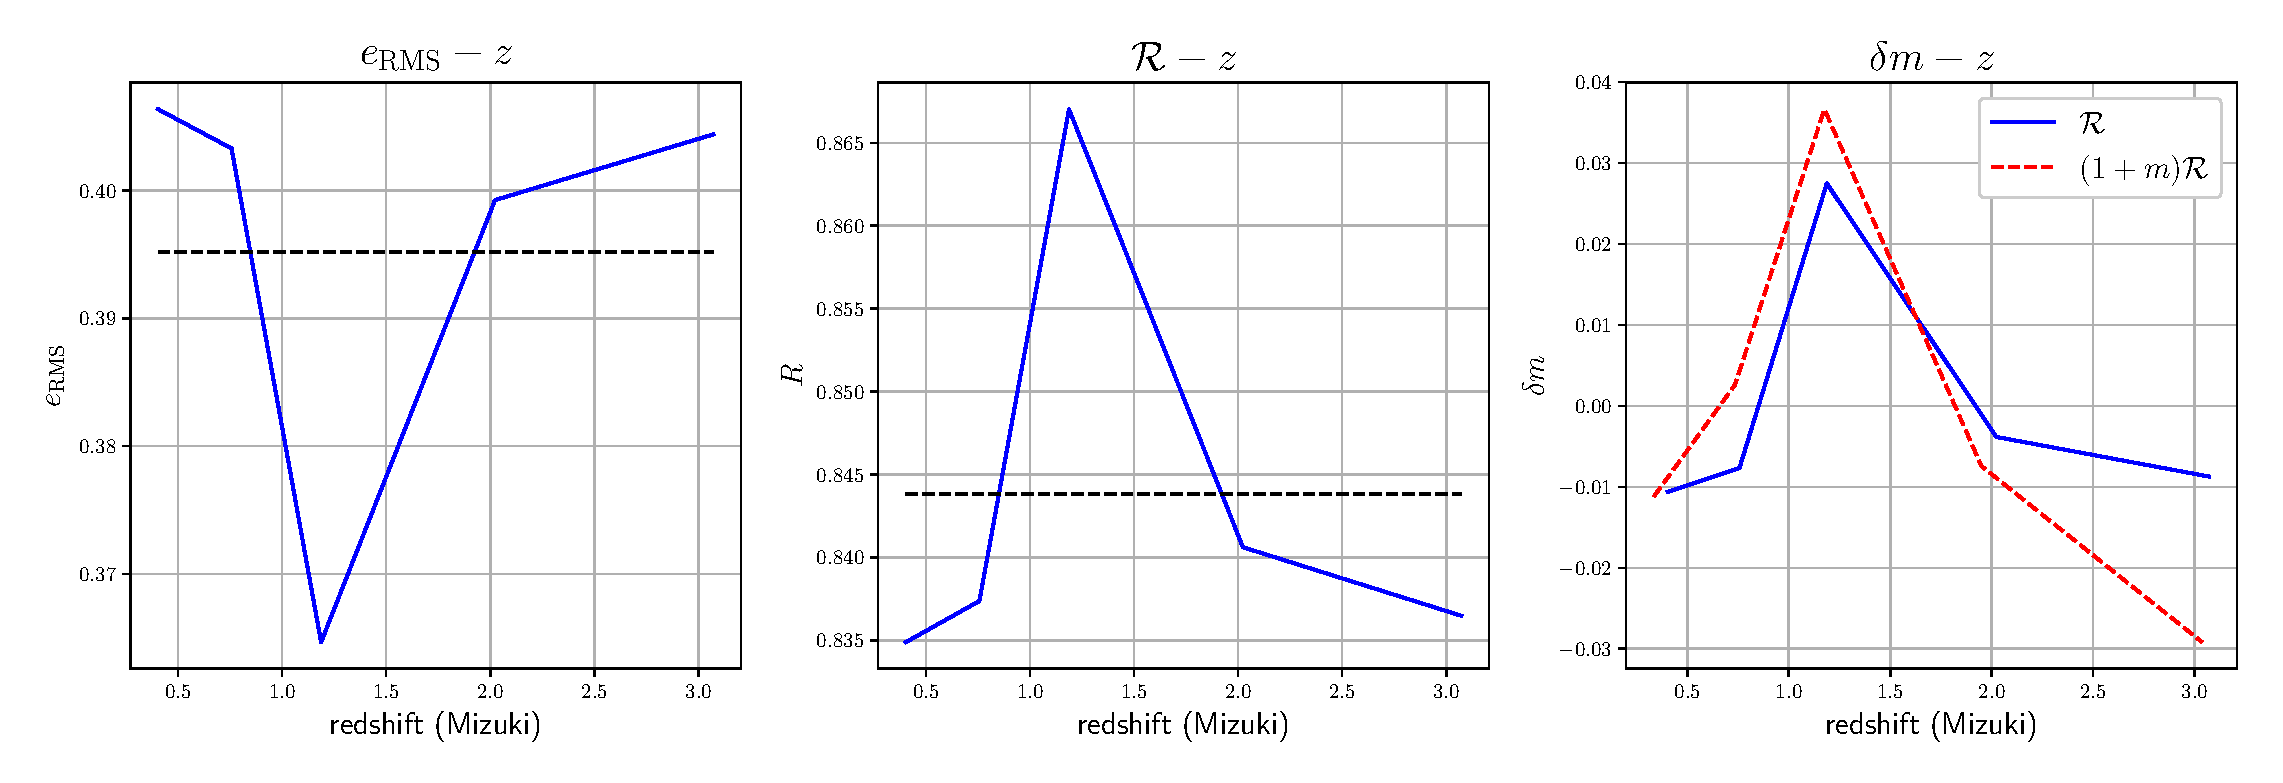
\includegraphics[width=0.9\textwidth]{redshift_dep_s16_vs_s19.eps}
}
\caption{The solid line in the left panel shows the redshift dependence of
    intrinsic shape and the dashed line in the left panel shows the average
    intrinsic shape. The solid line in the middle panel shows the redshift
    dependence of responsivity and the dashed line in the middle panel shows
    the average responsivity. The solid line shows in the right panel shows the
    multiplicative bias residual due to the redshift dependence of responsivity
    and the dashed line in the right panel shows the total multiplicative bias
    residual.
    }
\end{figure*}
